\documentclass[a4paper,11pt]{article}

\usepackage[utf8]{inputenc}

\usepackage{graphicx}
\usepackage{caption}
\usepackage{subcaption}

\usepackage{pgfplots}
\usepackage{float}
\usepackage{hyperref}
\usepackage{soul}
\hypersetup{
    colorlinks=true, % Enable colored links
    linkcolor=black, % Color for internal links
    urlcolor=black,  % Color for external links
    citecolor=black, % Color for citation links
    pdfborder={0 0 0}, % Remove border around links
}
\newcommand{\underlinehref}[2]{%
    \href{#1}{\ul{#2}}%
}
\pgfplotsset{compat=1.18}


\usepackage{minted}

\begin{document}

    \title{
        \textbf{The Stack in C}
    }
    \author{Péter Herczku}
    \date{Fall 2024}

    \maketitle

    \section*{Introduction}

    The task is to build up the Stack data structure from scratch and develop an HP-35 Calculator that uses the reverse Polish notation.
    I did the assignment in the C programming language.

    \section*{The stack}

    A stack is a data structure that allows us to {\tt push} and {\tt pop} elements from it.
    It works on the Last in, First out (LIFO) principle: the last element inserted is the first to be removed.
    The {\tt push} operation pushes an element to the end of the stack, and the {\tt pop} removes the last element of the stack.
    We distinguish two kinds of stacks, there is the static stack, where you need to specify the maximum amount of elements that it can hold, and there is the dynamic stack which grows as needed.
    Both kinds have their own use-cases, and we will look into that as well.

    \subsection*{Static stack}

    First, we will look at the static stack, because it is easier to implement.
    When we create a static stack we are actually allocating memory for an array with n elements.
    A static stack has a fixed sized, meaning its capacity cannot be extended.
    We also need to keep track of the stack pointer which points to the top of the stack (the next empty slot).
    However, in this case we have a problem: what happens when we try to push to a stack that is already full?
    We need to handle this problem and there are multiple ways of doing this.
    We can cancel the operation and throw an error to the user.
    This means that we cannot push onto our stack without popping an element first.
    \begin{minted}{c}
    void push(stack *stk, int val) {
        if(stk->top == stk->size) {
            printf("Stack overflow")
            return;
        }
        stk->array[stk->top] = val;
        stk->top++;
    }
    \end{minted}
    We also need to consider what happens when we try to pop an element from an empty stack.
    The solution is similar: we either throw an error to the user or return an unusual value from which the user knows that the stack is empty and there are no elements to be popped.
    After benchmarking, we see that the operations ({\tt pop, push}) run in constant time $O(1)$.

    \begin{figure}[h]
        \centering
        \begin{subfigure}[b]{.5\textwidth}
            \centering
            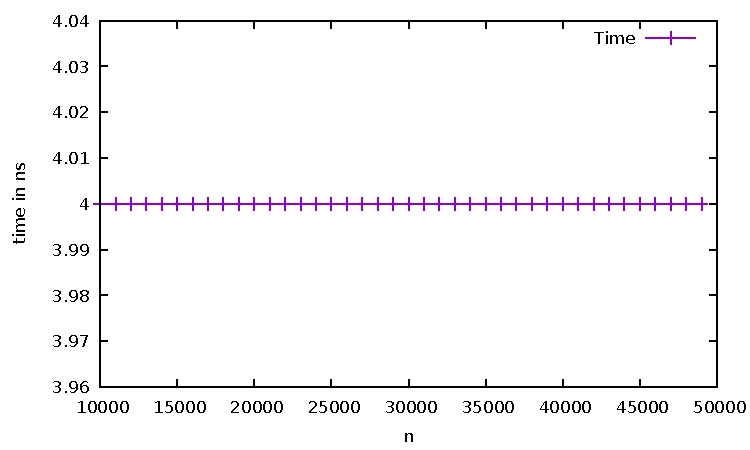
\includegraphics[width=\textwidth]{./static/data} % Adjust width or height as needed
        \end{subfigure}
        \caption{Graph of the time complexity of pushing and popping elements from stacks with different sizes}
        \label{fig:graph_1}
    \end{figure}

    But what if we don't know the size of the stack beforehand?
    We cannot just create a large empty stack, because we would waste a lot of memory.
    That's why we came up with the idea of dynamic stacks.

    \subsection*{Dynamic stack}

    As mentioned earlier, a dynamic stack is a stack that can grow as we add more elements.
    We handle this in the push operation: we need to check if the stack pointer had reached the top of the stack.
    If it had, then we need to extend the stack: we can extend it by a hundred elements for example.
    After benchmarking this solution, we can see that it is very expensive to do it this way.
    This may be negligible on smaller stacks, but it becomes costly as the stack grows.
    Let's take a look at another solution, we can double the size of stack every time we reach the end of it.

    \begin{minted}{c}
    if (stk->top == stk->size) {
        int size = stk->size * 2;
        int *copy = (int*) malloc(size*sizeof(int));
        for (int i = 0; i < stk->size; i++) {
            copy[i] = stk->array[i];
        }
        free(stk->array);
        stk->size = size;
        stk->array = copy;
    }
    stk->array[stk->top] = val;
    stk->top++;
    \end{minted}

    This way, our solution has roughly the same runtime as a static stack.
    To avoid memory leaks, we also need to shrink the stack as we pop elements from it.
    A common way of doing this is when the stack pointer reaches $n/4$, we set the size of the stack to $n/2$.
    \begin{minted}{c}
    if(stk->size > 4 && stk->top <= stk->size / 4) {
        int size = stk->size / 2;
        int* array = (int*) malloc(size * sizeof(int));
        for (int i = 0; i < size / 2; i++) {
            array[i] = stk->array[i];
        }
        stk->size = size;
        free(stk->array);
        stk->array = array;
    }
    \end{minted}

    \subsection*{More on memory management}
    We can see that the main challenge of dynamic stacks is memory management.
    Doubling the size of the stack is the most common approach since it provides a constant time complexity for the push operation, but we waste a significant amount of memory in edge cases.
    Let's say we have a dynamic with $10^5$ elements, but we want to add one more to it.
    We double the size, and waste a lot of useful memory.
    These are trade-offs that need to be considered depending on our use-case.

    \section*{Static or Dynamic stack?}

    The static stack provides better performance and predictable memory usage, but we sacrifice the ability to extend the stack when we need more capacity, which means that we need to implement it in our code by ourselves.
    On the other hand, dynamic stacks are a bit slower but give us more flexibility, and they are easier to work with.
    As you can see, this debate is not so simple, our choice depends on our use-case.
    For the calculator we are going to use the dynamic stack, because we have no idea how long our calculation is going to be.
    It would be hard to guess how large stack we should allocate and how to manage things when our stack overflows.

    \section*{The HP35 Calculator}

    If we look at the HP35 Calculator's implementation it is screaming that we should use a stack for this purpose.
    The calculator uses the {\tt reverse Polish notation}.

    \subsection*{What is the reverse Polish notation?}

    It's a mathematical notation where the operator is at the last place.
    This notation avoids using parenthesis, making the evaluation easier for computers.
    Example: {\tt 3 + 5} = {\tt 3 5 +}

    \subsection*{Back to the calculator}
    When we enter a number to the calculator it pushes it onto the stack.
    We keep doing this until we reach an operand, in that case we pop 2 elements and complete the operation on them, and we push back the result.
    When we reach the end of the operation, pressing enter pops the last the element from the stack, which is indeed our result.
    Now, let's calculate the result of:
        {\tt4 2 3 * 4 + 4 * + 2 -}
    The result is 42.

    \section*{GitHub}
    I have uploaded the full project to \underlinehref{https://github.com/peterherczku/ID1021/tree/main/assignment-2}{my github repository}, where we can find the code used to make this report.

\end{document}
